\documentclass[default,pdf,colorBG,slideColor]{prosper}
\usepackage{epsfig}
\usepackage{pstricks}
\usepackage{graphicx}

\graphicspath{ {../fig/} }

\title{Next Generation Resource Manager}
\subtitle{{\small high level technical review}}
\author{Dong Ahn, Jim Garlick, Mark Grondona, Don Lipari}
\email{{\rm \{ahn1,garlick,mgrondona,lipari\}@llnl.gov}}
\institution{Livermore Computing \\
             Lawrence Livermore National Laboratory}

\slideCaption{NGRM High Level Review, Mar. 4, 2013}

\Logo(-1,-1){
\epsfig{file=graphic/iccd_logotrans.ps,scale=0.15}}

%\Logo{
\includegraphics[scale=0.15]{iccd_logotrans.ps}}


\begin{document}

% ==========================================================================
\maketitle
% ==========================================================================
\begin{slide}{Session Overview}{\small
We will roughly follow the outline of the {\em Vision} document.\\
\begin{itemize}
  \item[\S1-4]{{\em overview} (Jim)}
  \item[\S5]{{\em comms framework} (Jim)}
  \item[\S6.1-6]{{\em resource management} (Mark)}
  \item[\S6.7]{{\em scheduler} (Don)}
  \item[\S7]{{\em monitoring} (Jim)}
  \item[\S8]{{\em runtime} (Dong)}
\end{itemize}
We expect to address your questions and comments as we go.
}\end{slide}
% ==========================================================================
\part{overview}
% ==========================================================================
\begin{slide}{RM today}{\small
Here describe slurm emphasising its design space, scalability
limitations, node-centric resource model, etc..  What is good about slurm
that we would like to carry fwd.
}\end{slide}
% ==========================================================================
\begin{slide}{vision and new capabilities}{\small
\begin{itemize}
  \item{center as a cluster}
  \item{diverse compute resources}
  \item{data provenance and reproduceability}
  \item{low noise}
  \item{fault tolerance}
  \item{security}
  \item{research and tool friendly}
  \item{extensibility}
\end{itemize}
}\end{slide}
% ==========================================================================
\begin{slide}{design challenges}{\small
\begin{minipage}{0.45\textwidth}
\begin{itemize}
  \item{multidimensional scale challenge}
  \item{diverse workload challenge}
  \item{dynamic workload challenge}
  \item{power challenge}
  \item{scheduling challenge}
\end{itemize}
\end{minipage}
\begin{minipage}{0.45\textwidth}
\begin{itemize}
  \item{backwards compatibility challenge}
  \item{integration risk}
  \item{higher downtime costs}
  \item{separation-of-concerns challenge}
  \item{security challenge}
  \item{productivity challenges}
\end{itemize}
\end{minipage}
}\end{slide}
% ==========================================================================
\begin{slide}{new conceptual models}{\small
\begin{itemize}
  \item{unified job model}
  \item{job hierarchy model}
  \item{generalized resource model}
  \item{resource allocation elasticity model}
  \item{common scalable infrastructure model}
  \item{self-hosting model}
  \item{lightweight virtualization model}
\end{itemize}
}\end{slide}
% ==========================================================================
\begin{slide}{Next Generation Resource Manager}{\small
insert {\em vision} figure 2 job hierarchy (several slides showing
progression.
}\end{slide}
% ==========================================================================
\begin{slide}{job 0}{\small
\begin{center}
  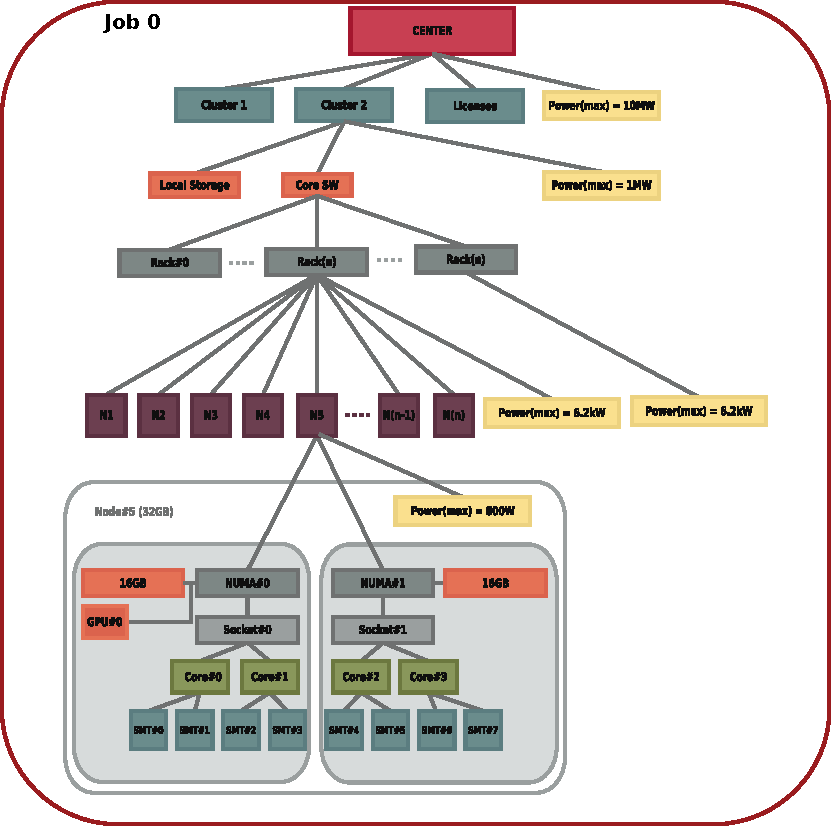
\includegraphics[scale=0.50]{job-hierarchy-job0}
\end{center}
}\end{slide}
% ==========================================================================
\begin{slide}{job 0.x}{\small
\begin{center}
  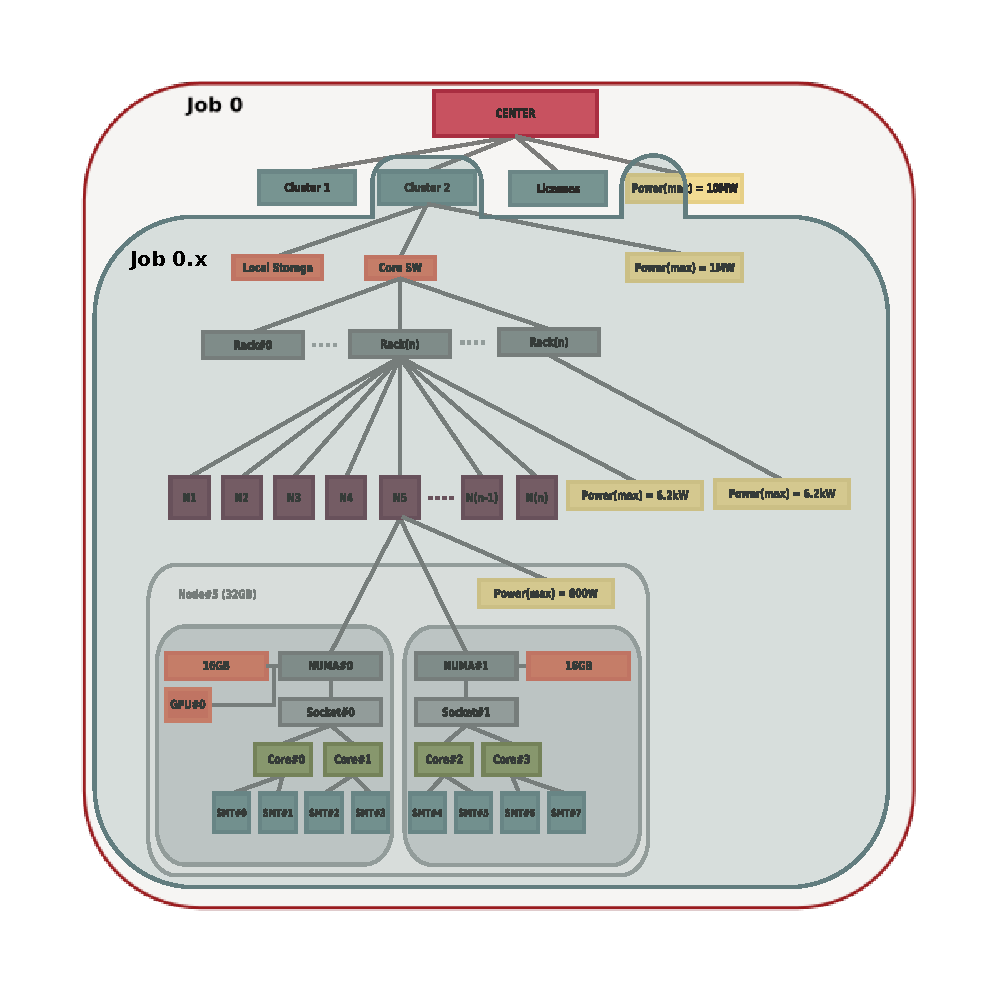
\includegraphics[scale=0.50]{job-hierarchy-job0-x}
\end{center}
}\end{slide}
% ==========================================================================
\begin{slide}{job 0.x.y}{\small
\begin{center}
  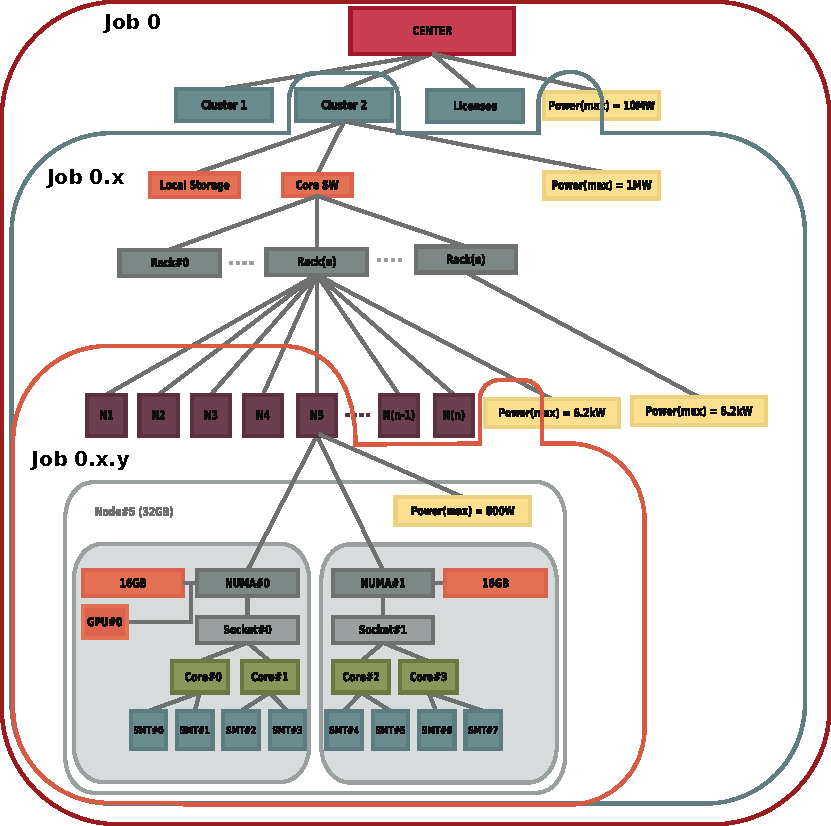
\includegraphics[scale=0.50]{job-hierarchy-job0-x-y}
\end{center}
}\end{slide}
% ==========================================================================
\begin{slide}{comparision with slurm}{\small
\begin{itemize}
  \item{job}
  \item{job step}
  \item{reservations}
  \item{job accounting}
\end{itemize}
}\end{slide}
% ==========================================================================
\begin{slide}{project organization and thrust areas}{\small
\begin{itemize}
  \item{comms framework}
  \item{resource management}
  \item{monitoring}
  \item{runtime}
\end{itemize}
Add sub-lists to break each down a bit
}\end{slide}
% ==========================================================================
\part{comms framework}
\part{resource management}
\part{scheduler}
\part{monitoring}
\part{runtime}
% ==========================================================================
\end{document}
